\documentclass[../main.tex]{subfiles}
\graphicspath{{\subfix{../images/}}}
\begin{document}


\index{stress!definition}
The formal definition of Stress is the attempt of the body to get back to equilibrium (homeostasis)\index{homeostasis} as fast as possible after an irritating stimulus.
There's a distinction to be made between negative stress which get caused by ``seeming impossible''
 situations and positive stress caused in situations which are subjectively perceived as surmountable.
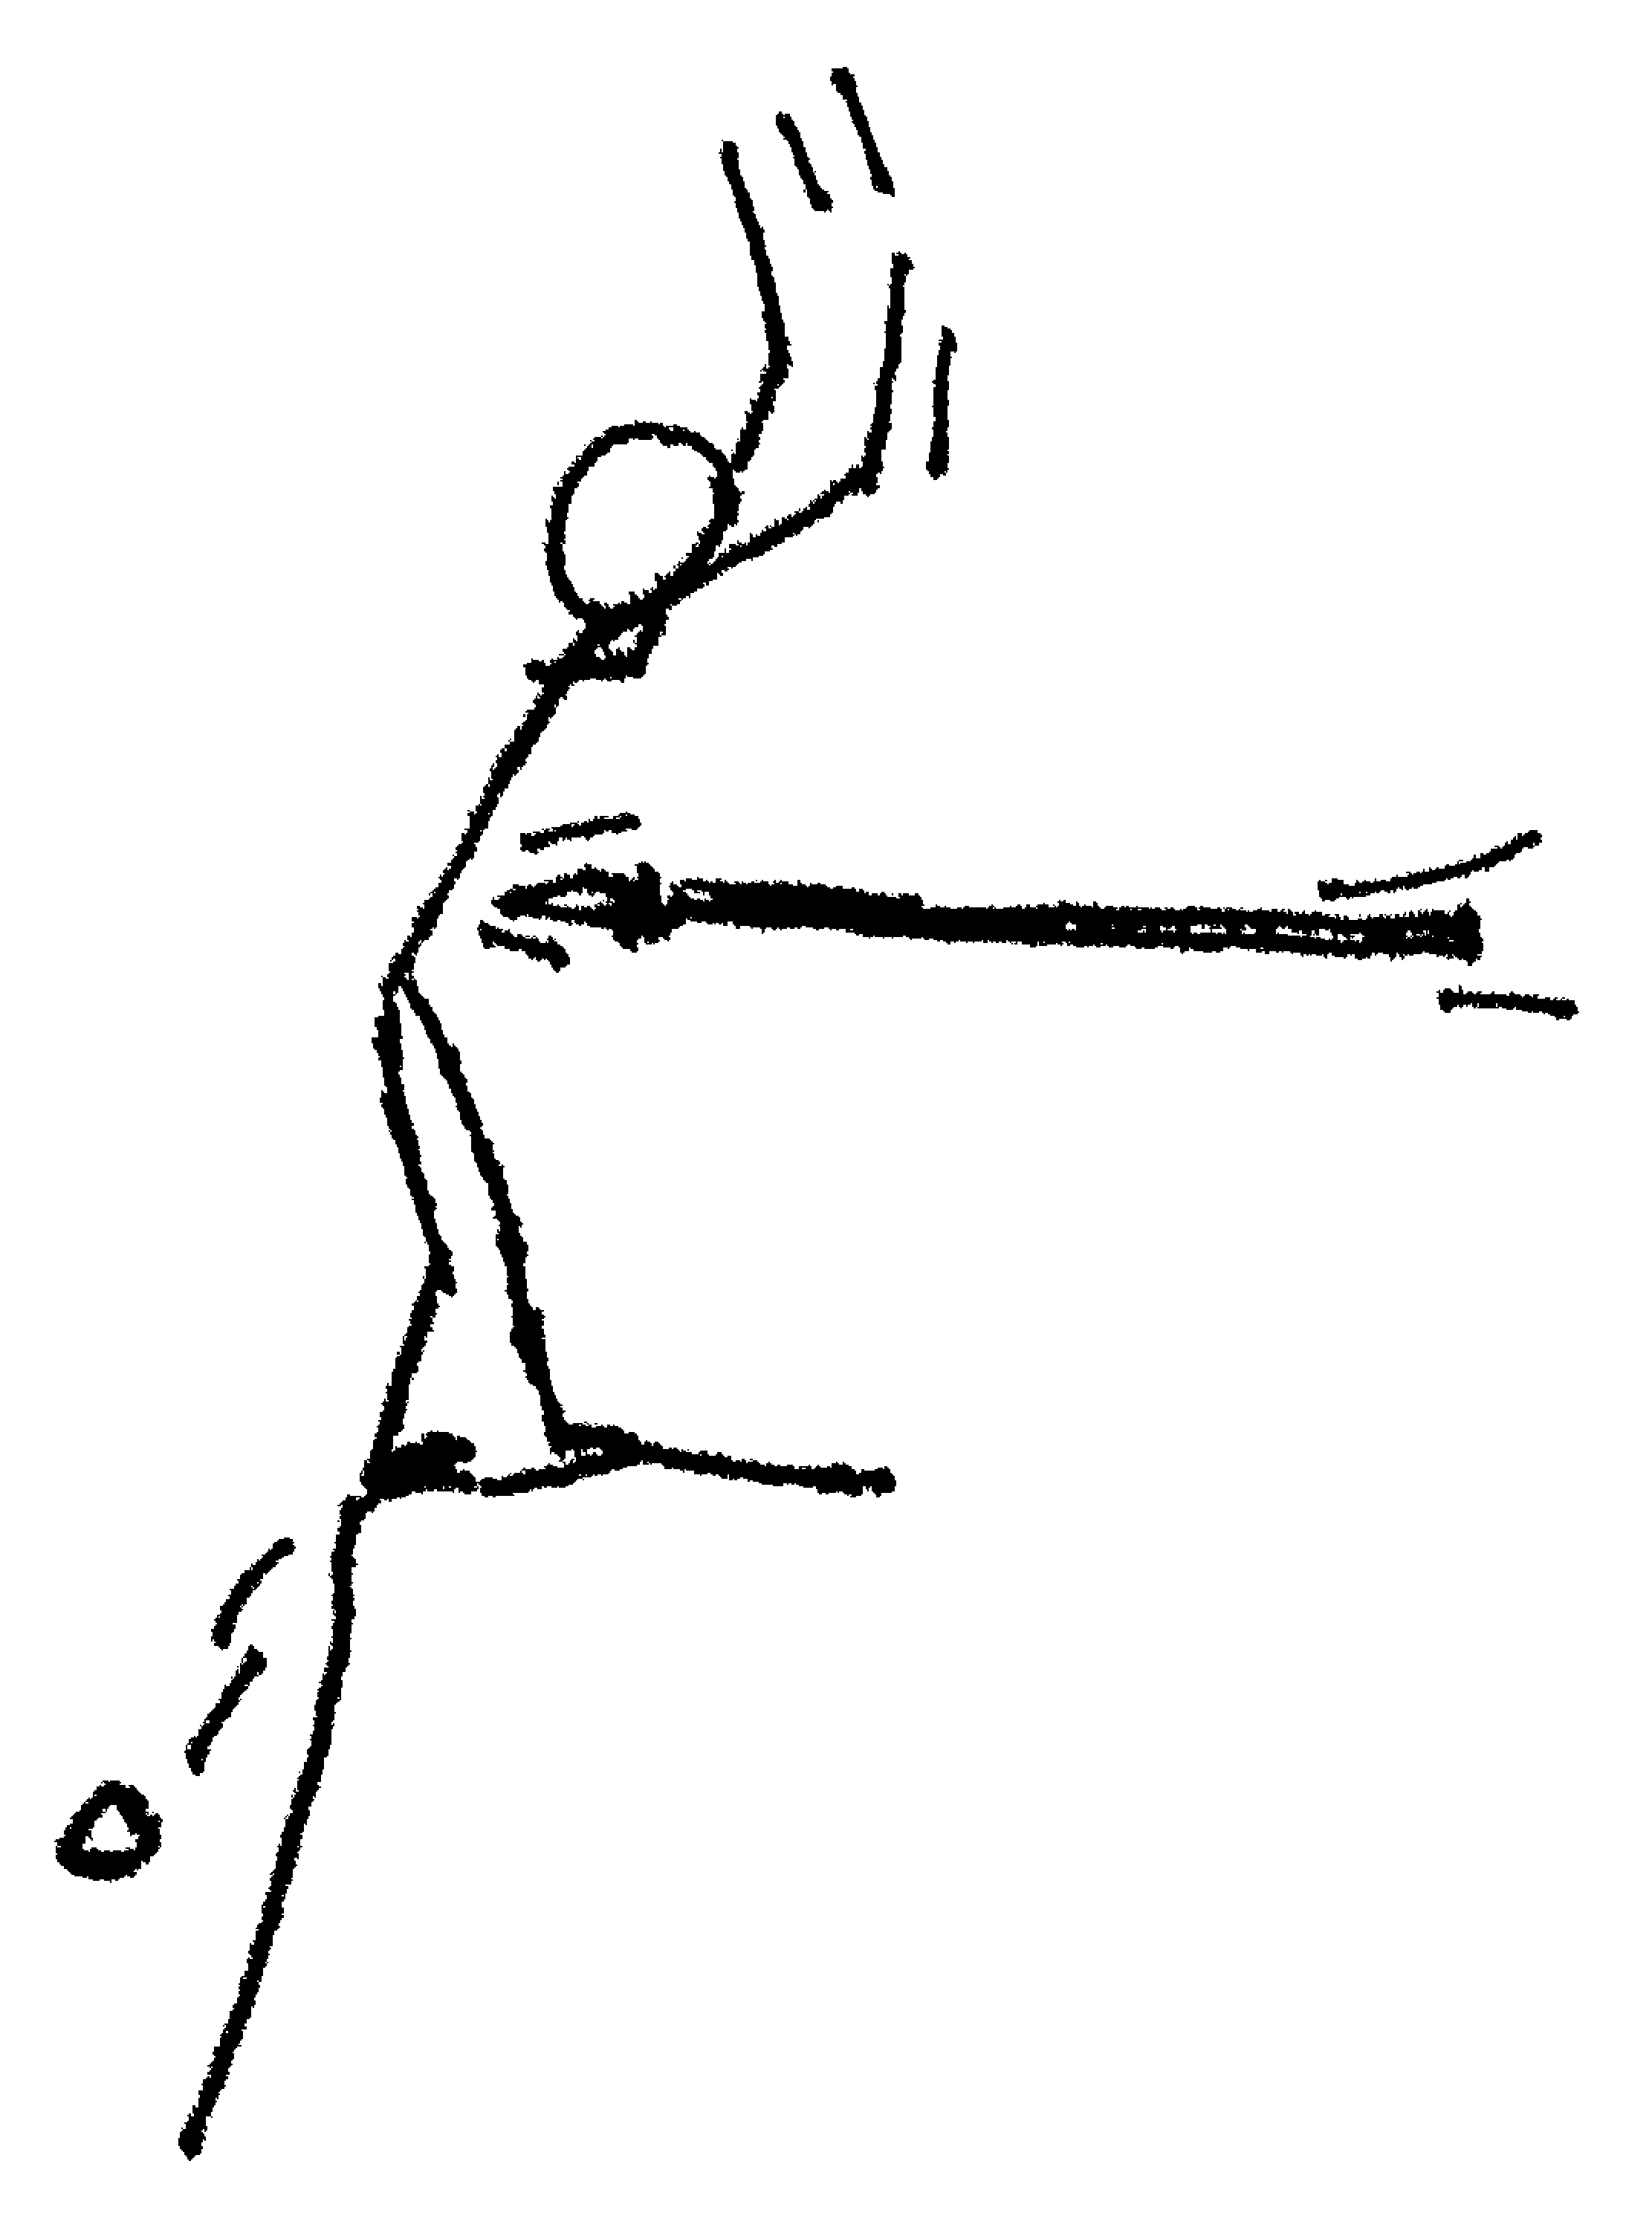
\includegraphics[width=3cm]{Guy-Edge}

Humans can't live without stress, for many situations it needs a heightened action potential. For instance stress releases the stress hormones in the body. They trigger diverse reactions in the body: the hearth rate increases, brain and lungs get better supplied and the senses get sharpened.

The term stress\index{stress!definition} was introduced 1936 by the Austrian-Canadian doctor Hans Selye\index{Selye, Hans} to describe the \emph{reaction of biological systems to pressure}. The term was meant to neutrally describe what happens in the body in such situations.
It's important to note, that it didn't have the negative connotation yet, that nowadays is often attributed to the term but in it's original meaning it should neutrally describe what happens to the body when it is under pressure.

\subsubsection{Is Stress Needed?}

This question is less harmless than it looks like. First of all, we have to distinguish between two types of stress:
	\begin{description}
		\item[Negative Stress]\index{stress!negative} triggered by ``seemingly impossible situations''
		\item[Positive Stress]\index{stress!positive} triggered in situations which are subjectively perceived as manageable
	\end{description}
	
Humans couldn't possibly live without stress. Stress is a necessary ingredient for a human's ability to thrive and grow on obstacles. It produces an heightened action potential, which is needed in many situations.

Nowadays, the expression stress is the general term for the mental and bodily reactions to inner or outer impulses, which humans perceive as pleasant or as burdening.
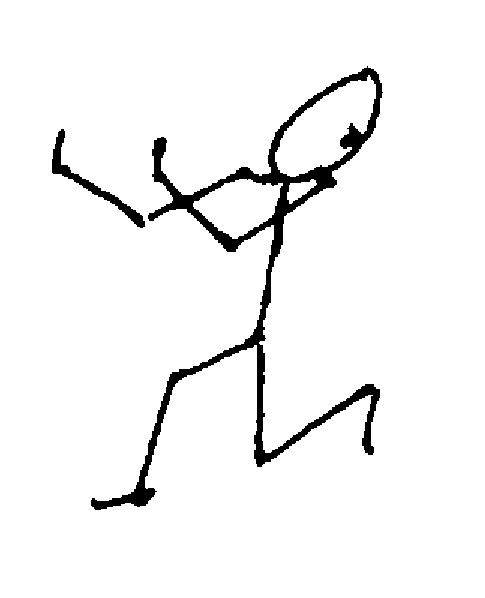
\includegraphics[width=2cm]{Guy_Distress}
\hspace{5cm}
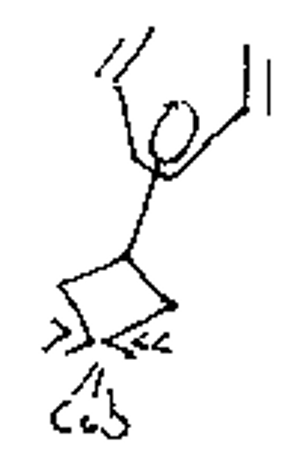
\includegraphics[width=2cm]{Guy_Eustress}

\section{Eustress vs. Distress}

\emph{Eu--stress}\index{Eustress (Eu--stress)} (Greek ``Eu'' = ``good'') is exciting stress and vital for humans. 
Eustress is a situation, which we perceive as increasing our well--being. 

On the other hand, \emph{Dis--stress}\index{Distress (Dis--stress)} (Greek ``dis'' = ``against'') is life endangering stress. In this situation we feel a burden or pressure from inside or outside.



\epigraph{Life isn't about waiting for the storm to pass \ldots  \\ 
It's about learning to dance in the rain.}{\textit{Anonymous}, more recently attributed to \textit{Vivian Greene}}


\subsubsection{Conclusion}
\noindent In light of the distinctions we made, let's talk about the best stress regulation measure\index{stress!regulation} possible:
\begin{itemize}
\item Distress (Dis--stress) can be changed to eustress with appropriate methods, taking into account the individual tenacity and sensitivities.
\item As soon as we realize that we decide ourselves about the perception of pleasurable stress (eustress) and painful stress (distress) we get our freedom back. 
\item The taxing stress has to be let go on a conscious level. Many people think they are in stress but aren't, and the other way round.
\end{itemize}

\epigraph{Human: learn to dance, so when you get to heaven the angels know what to do with you.}{\textit{St. Augustine}}


%------------------------------------------------
\end{document}